\chapter{Maximizing Utility in Motion Planning}
\label{chap:utility}

\cdnote{This was the abstract:}

Faced with articulated motion tasks in semi-structured environments,
autonomous robots must allocate limited resources between planning
motions and subsequently executing them.
Existing approaches for motion planning in such high-dimensional
spaces,
including sampling-based, asymptotically optimal and anytime planners,
risk either quickly returning a solution that is expensive to execute,
or spending too much planning effort improving an existing solution.
Our primary contribution is to imbue 
lazily-evaluated sampling-based approaches
with a \emph{utility function}
which incorporates both planning and execution cost in its objective.
Reasoning over utility provides the planner
with a means to trade off between these costs using a single input
parameter,
as well as a natural termination condition.
Furthermore,
treating planning cost explicitly
provides a natural way to accommodate task-specific planning
heuristics.
The planner performs well on a set of benchmark tasks,
and is particularly amenable to caching
%\scnote{Is caching a standard thing in the roadmap planning context?
%Or if not, do you intend to explain it further?}
and parallelization.
We also discuss a configuration space decomposition
and accompanying planning cost model
for multi-step manipulation planning tasks.

\section{Introduction}

\scnote{General Comment: I did not quite follow how 'marginal' utility applies here. I'm sure it is not the term from probability.
Do you use marginal to indicate that you optimize for utility?}

Autonomous robots in the real world
must carefully allocate limited resources (e.g. time or energy)
between planning motions and executing them.
A robot that favors execution
risks prematurely committing to an uneconomical path, whereas
one that favors planning risks unduly delaying execution 
due to incessant small refinements.
This tradeoff is especially relevant for working with
or around humans, who are simultaneously 
unaccommodating of long pauses
and of wild and unpredictable motion.

Most planning algorithms pick a side and stick to it.

Randomized algorithms such as the
PRM~\citep{kavrakietal1996prm}
and RRT~\citep{lavallekuffner1999rrt},
strive to find feasible paths while minimizing planning cost,
falling in the $A_1$ category of the planning vs. execution
plot (Figure~\ref{fig:fig1}, we will formalize notation 
in Section \ref{sec:utility}).
Techniques such as caching, parallelization \citep{ichnowski2012prrt},
and lazy evaluation \citep{bohlin2000lazyprm}
are often used to further reduce online planning cost.
%They use post-processing like path 
%shortcutting to reduce execution effort albeit exclusively 
%focusing on minimizing planning effort.

Optimal algorithms
such as FMT*~\citep{janson2015fmtstar}
exclusively optimize for execution
cost ($A_2$ in Figure~\ref{fig:fig1}), 
and often use techniques such as informed heuristics to improve
planning efficiency as a secondary objective.
Graph search approaches \citep{hart1968astar}
can guarantee solution optimality
with respect to a chosen discretization,
and often incorporate a parameter ($A_3$) such as inflation
\citep{pohl1970weightedastar}
or an execution cost bound \citep{stern2014}
that reduces the algorithm's runtime at the expense of optimality.
However,
it can be difficult to set these parameters for a particular domain.

Anytime algorithms $A_4$
for continous
\citep{karaman2011samplingoptimal, gammell2015bitstar, hauser2015lazy}
or discrete
\citep{likhachev2004arastar} problems
come the closest, providing a sequence of solutions
with decreasing execution cost.
However, they are best suited for \emph{uncertain}
planning budgets, and as a consequence of this uncertainty
incur planning cost producing
solutions that never get used.
It can also be difficult to decide when to terminate them.
We wish to do better.

\begin{figure}
   \centering
   \begin{tikzpicture}
      \node[inner sep=0cm] at (1.9,6.25) {\includegraphics{build/pvx-graph}};
      \node[inner sep=0cm] at (2.08,2.65) {\includegraphics[width=3.51cm]{build/multiple-sets}};
      \node[inner sep=0cm] at (6.5,4.77)
         {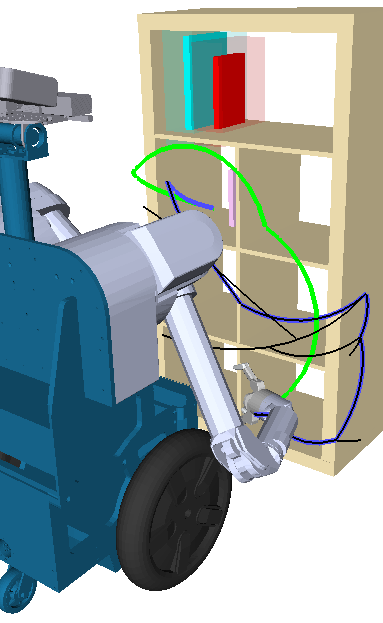
\includegraphics[width=4.25cm]{figs/herbarm-snapshot-cropped.png}};
         
      \node[fill=white,inner sep=2pt,anchor=west] at (7.5,7.5) {\scriptsize planning: 2.9s};
      \node[fill=white,inner sep=2pt,anchor=west] at (7.5,7.2) {\scriptsize execution: 5.7s};
      \draw[thick,->] (7.5,7.35) -- (7.0,6.5);
      
      \node[fill=white,inner sep=2pt,anchor=west] at (7.0,2.0) {\scriptsize planning: 2.4s};
      \node[fill=white,inner sep=2pt,anchor=west] at (7.0,1.7) {\scriptsize execution: 12.4s};
      \draw[thick,->] (7.8,2.2) -- (8.05,3.2);
   \end{tikzpicture}
   \caption[]{
      A robot reaching to grab a book
      must allocate limited resources between planning and executing its motion.
      Our planner reasons over a user-defined utility function (top~left)
      to explicitly trade-off between these two significant sources
      of cost.
      As its roadmap search (right) discovers valid edges
      (\protect\tikz{\protect\draw[thick] (0,0) -- (0.15,0.15);}),
      it mediates between
      high-cost edges that are fast to find~%
      (\protect\tikz{\protect\draw[blue,ultra thick] (0,0) -- (0.15,0.15);})
      and low-cost edges that require significant planning~%
      (\protect\tikz{\protect\draw[green,ultra thick] (0,0) -- (0.15,0.15);})
      directly via their prospective utilities.
      Because the planner accepts arbitrary estimators
      for planning cost,
      it can naturally exploit both caching and geometric structure in
      $\mathcal{C}$ (bottom left).
      \cdnote{Turns out the right HERB example is not a great one
      -- I'll look for a better one tomorrow
      (and improve the figure quality itself).}
      \cdnote{Replace bottom-left with fancy 3D plot?}}
   \label{fig:fig1}
\end{figure}

Our goal is to devise an algorithm that \emph{explicitly} reasons over both planning
and execution cost. Our algorithm should behave like an optimal algorithm 
if execution cost is critical, and like a randomized algorithm if planning
cost is critical. Crucially, it should behave like a mix between the two 
if both are important to the user.

To enable this, we borrow a concept from the AI community~\citep{ruml2007bugsy},
allowing the user to specify a \emph{utility function} describing
their planning vs. execution tradeoff
(illustrated via isocontours in Figure~\ref{fig:fig1}).
We describe some examples and theoretical properties of this
function in Section \ref{sec:utility}, but it can be arbitrarily nuanced, 
or extremely simple,
e.g. a linear function that sums planning and execution cost.
We argue that utility is an essential metric
by which to evaluate motion planners.

Considering this utility function, we make the following observations: 
(1) we can update estimates of utility online during planning;
(2) we can estimate execution cost of a path
(e.g. path length or energy) quite accurately.
%\scnote{The idea I get reading is that it is the utility 
%function that lets you estimate execution cost quite accurately, which I guess
%is not the idea.}.

However, our key insight is that we can
\emph{estimate the planning cost} in domains
where this cost is dominated by the effort of
verifying the validity of edges via collision-checking.
This is true for most real-world robot motion planning problems
where 80-95\% of the planning time
is dominated by collision-checking.

When combined, these insights enable a planning approach which
reason explicitly over utility using online estimates.
This leads naturally to the
Lazily Evaluated Marginal Utility Roadmaps (LEMUR) planner
(Section~\ref{sec:roadmaps}).
LEMUR takes as input a parameterized utility function $U_\lambda$ 
and attempts to find and validate a solution path
that maximizes that utility.

LEMUR has several advantages over anytime planners.
First,
the user's utility function provides a natural termination condition
-- the planner returns a solution when no alternatives provide
a prospective improvement in utility.
Second, the planner does not waste effort generating
intermediate solutions.

The performance of LEMUR is also easier to tune to a particular
problem domain.
In particular,
the parameter it uses to mediate between costs is
the user's utility function itself.
It is therefore unnecessary to tune inflation factors or
trajectory optimization budgets to achieve good performance.

We compare LEMUR to several sampling-based and anytime planners
across a set of motion planning problems
in Section~\ref{sec:experiments}.

LEMUR's ability to accept an arbitrary planning effort model
enables it to be customized to different domains.
In Chapter \ref{chap:family},
we discuss such a model specific to problems over a family of
C-space subsets.
A prime example of this is multi-step manipulation tasks
in which the C-space changes with each object grasp and placement.
This allows computation to be efficiently cached and reused.

The combination of
marginal utility, lazy evaluation, and roadmap methods
work in concert and are adaptable to new domains.
Section~\ref{sec:discussion} concludes the paper with a discussion
of potential extensions and applications of our algorithm.

\section{Utility in Motion Planning}
\label{sec:utility}

We consider the motion planning problem in a configuration space
$\mathcal{C}$:
given the collision-free subset
$\mathcal{C}_{\ms{free}} \subset \mathcal{C}$
and configurations
$q_{\ms{start}}$ and $q_{\ms{goal}}$,
find a valid path
$\xi: [0,1] \rightarrow \mathcal{C}_{\ms{free}}$
with $\xi(0) = q_{\ms{start}}$
and $\xi(1) = q_{\ms{goal}}$.
We further consider a cost function
$x: \Xi \rightarrow \mathbb{R}^+$
which measures path quality --
in our case, the cost of executing a solution path.
Examples of $x$ include the path's length
or the time or energy required to execute it.
$x$ is commonly treated as part of the problem specification;
each instance admits a path(s) with optimal execution cost $x^*$.

A sound motion planner $A$ accepts a problem instance
and yields a valid solution path $\xi$
with execution cost $x(\xi)$.
We are also interested in measuring the planning cost incurred by
the algorithm itself
via a real-valued performance metric $p$.
Examples of $p$ include the number of iterations or
collision checks performed,
or the amount of time or energy consumed by the planner.
Figure~\ref{fig:utility-contours} provides an illustration of
these two costs on the plane.

In general,
a planner endeavoring to reduce the execution cost of its solution path
must incur additional planning cost to do so.
While a wealth of planning approaches are available in the literature,
few attempt to capture this underlying tradeoff directly.
We propose to do so via a \emph{utility function}.
Utility functions were first exploited by the
Best-first Utility-Guided Search (BUGSY) algorithm
\citep{ruml2007bugsy,burns2013bugsy}
to order vertex expansions during a
conventional graph search.
We propose to apply a similar insight to motion planners
which use lazy evaluation.

\subsection{Utility Functions}
\label{subsec:utility-functions}

A utility function $U$ is a scalar-valued function
over both $p$ and $x$
which provides the motion planner with
the \emph{utility} of returning a
solution path with execution cost $x$ calculated after
incurring planning cost $p$
(Figure~\ref{fig:utility-contours}).
Utility functions are applicable to a wide range of planning regimes
and often emerge readily from the problem domain.
A utility function also naturally reconciles cost functions
$p$ and $x$ that are in different units
(e.g. collision checks and path length).
We follow the convention that utility is to be maximized
(whereas cost is to be minimized).

\begin{figure}
   \centering
   \subfloat[A utility function over $p,x$]{%
      \centering
      \includegraphics{build/pvx-utility}
      \label{fig:utility-contours:pvx-utility}
   }%
   \quad%
   \subfloat[Maximizing utility with parameterized or anytime planners]{%
      \centering
      \includegraphics{build/pvx-utility-anytime}
      \label{fig:utility-contours:pvx-utility-anytime}
   }%
   
   \subfloat[First feasible]{%
      \centering
      \includegraphics{build/pvx-sm-firstfeas}
      \caption{}
      \label{fig:utility-contours:pvx-sm-firstfeas}
   }%
   \quad%
   \subfloat[Bounded cost]{%
      \centering
      \includegraphics{build/pvx-sm-xbudget}
      \label{fig:utility-contours:pvx-sm-xbudget}
   }%
   \quad%
   \subfloat[Planning budget]{%
      \centering
      \includegraphics{build/pvx-sm-pbudget}
      \label{fig:utility-contours:pvx-sm-pbudget}
   }%
   \caption{Contours of a utility function $U(p,x)$.
      Also some examples of simple utility functions
      relevant to related work.}
   \label{fig:utility-contours}
\end{figure}

While $U$ may be any function,
there are certain properties that we can expect from any reasonable
choice.
In particular,
\begin{equation}
   \nabla U \leq \mathbf{0}.
\end{equation}
This follows from the following arguments
(Figure~\refsub{fig:utility-contours}{pvx-utility}).
If $\partial_x U$ were positive,
it would be beneficial for a planner to return a path with larger
execution cost.
Similarly,
if $\partial_p U$ were positive,
it would be beneficial for a planner to artificially delay returning
a given solution path.

\cdnote{Say something about local structure, dot product, etc etc.}

Several common planning regimes can be expressed exactly as
utility functions.
For example,
requesting a planner to return a solution as quickly as possible
irrespective of its execution cost corresponds to the first-feasible
utility in Figure~\refsub{fig:utility-contours}{pvx-sm-firstfeas}.
Bounded-cost planners such as Potential Search (PTS) \citep{stern2014}
address problems in which a solution below a prescribed cost $x_b$ is
desired as quickly as possible (Figure~\refsub{fig:utility-contours}{pvx-sm-xbudget}).
The converse formulation requests the lowest-cost path
within a fixed planning budget $p_b$
(Figure~\refsub{fig:utility-contours}{pvx-sm-pbudget}).

It is instructive to consider how existing types of planners
might be applied if utility is to be maximized.
Many planners
($A_3$ in Figure~\refsub{fig:utility-contours}{pvx-utility-anytime})
take parameters which profoundly affect both the
quality of their solutions and the planning cost they incur.
The range parameter of the RRT \citep{lavallekuffner1999rrt}
and the inflation factor in Weighted A* \cite{pohl1970weightedastar}
are common examples of this.
However,
it is difficult to choose the values for these parameters;
they must often be learned empirically in a way that is
specific both to the planner and to the problem instance.

Anytime planners such as
Anytime Repairing A* \citep{likhachev2004arastar}
and RRT* \citep{karaman2010rrtstar}
return a low-quality solution quickly,
and then continually return improved solutions as more planning
is performed ($A_4$ in Figure~\refsub{fig:utility-contours}{pvx-utility-anytime}).
Applying an anytime planner to a utility-maximization problem suffers
from two drawbacks.
First,
an outside process must enforce an appropriate termination condition.
While this may be straightforward for simple utilities
(e.g. from Figures~\refsub{fig:utility-contours}{pvx-sm-firstfeas}-%
\refsub{fig:utility-contours}{pvx-sm-pbudget}),
a nontrivial utility function requires a complex termination model
which must be learned in a problem-specific way.
Second,
scarce planning resources are typically allocated on low-quality
intermediate paths which will go unused.

\begin{algorithm}[t]
\caption{Lazily Evaluated Utility-Guided Search Outline}
\label{alg:utility-search-outline}
\begin{algorithmic}[1]
\For {iteration $i \in 1, 2, \dots$}
   \State $\bar{p}_i \leftarrow$
      planning cost incurred so far
   \State $\Xi_i \leftarrow$ set of paths to consider at iteration $i$
   \State $\grave{p}_i : \Xi_i \rightarrow \mathbb{R}^+$
      \Comment additional planning cost estimator
   \State $\hat{x}_i : \Xi_i \rightarrow \mathbb{R}^+$
      \Comment execution cost estimator
   \State $\xi_i = \argmax_{\xi \in \Xi_i}
      U\!\left( \; \bar{p}_i \! + \! \grave{p}_i(\xi), \; \hat{x}_i(\xi) \; \right)$
      \label{line:outline-argmax}
   \State \Return $\xi_i$
      if $\grave{p}_i( \xi_i ) = 0$
   \State evaluate $\xi_i$
      \Comment incurs requisite planning cost
\EndFor
\end{algorithmic}
\end{algorithm}

\subsection{Outline of Lazily Evaluated Utility-Guided Search}

We endeavor to marry utility functions with lazy motion planning.
Lazy path evaluation is well-suited to domains with expensive
validity checking,
and is a common technique \citep{bohlin2000lazyprm, cohen2014narms}.
Here,
we provide the general outline of a class of algorithms which
takes as input a utility function $U$
and selects paths to evaluate based on estimates of their utility.

The planner maintains estimates $\hat{p}$ and $\hat{x}$
of the planning and execution costs, respectively,
for each of a set of prospective trajectories $\Xi$.
While a prospective path's execution cost may be easy for a planner
to estimate via commonly used heuristics,
incorporating estimates of the planning cost
to be incurred by the algorithm itself is more difficult.
While the planner is running,
we can decompose its planning estimate $\hat{p}$ for a prospective
path $\xi$ into two components:
\begin{equation}
   \hat{p}(\xi) = \bar{p} + \grave{p}(\xi)
\end{equation}
that is,
the measured planning cost elapsed $\bar{p}$
and the estimated remaining planning cost $\grave{p}$.

\begin{figure}
   \centering
   \subfloat[Planning cost estimates]{%
      \centering
      \includegraphics{build/p-estimates}
      \label{fig:pvx-linear-discounting:p-estimates}
   }%
   \quad%
   \subfloat[Evolution of path utilities]{%
      \centering
      \includegraphics{build/pvx-linear-discounting}
      \label{fig:pvx-linear-discounting:pvx-linear-discounting}
   }
   \caption{A planner reasoning with a linear utility function
      chooses to first evaluate trajectory $\xi_1$.
      After incurring planning cost $\bar{p}$
      (less than it had expected),
      it finds that it is more expensive than expected;
      some of the planning work has also adjusted the estimates
      for nearby trajectory $\xi_2$.
      However,
      the estimated remaining planning costs $\grave{p}$
      for all other unaffected trajectories have remained constant.
      Therefore, the relative utilities have also not changed.
      As such, a planner need not re-order any trajectories whose
      estimated planning cost to go has not changed.
      \cdnote{This explanation can be vastly improved.}}
   \label{fig:pvx-linear-discounting}
\end{figure}

Consider the planner outline in
Algorithm~\ref{alg:utility-search-outline}.
At each iteration $i$,
the planner has incurred $\bar{p}_i$ planning cost so far.
It considers a set of prospective paths $\Xi_i$
(left unspecified).
It also has available estimators for each path's execution cost
$\hat{x}_i$
and its remaining planning cost
$\grave{p}_i$.
Note that these estimators can change between iterations --
for example,
a path's remaining planning estimate becomes 0 once it is
fully evaluated,
and its execution effort becomes $\infty$ if it is found to be
infeasible.
Estimates for other paths which share segments may also be
updated (Figure~\ref{fig:pvx-linear-discounting}).
\scnote{Similar concern. At this stage I (as a new reader) am still having difficulty figuring out what 
exactly the planning effort implies, and understanding that they are related, might help that }

Using these estimators,
the planner selects among $\Xi_i$
the path $\xi_i$ which maximizes the given utility function $U$.
If no planning cost remains, it is returned;
otherwise,
it is evaluated,
incurring the requisite planning cost.
Note that this algorithm terminates naturally,
and therefore avoids incurring planning cost seeking out
low-quality intermediate solutions.

The outline in Algorithm~\ref{alg:utility-search-outline} is able to
broadly capture the behavior of a number of well-known planning
algorithms.
For example, consider the symmetric bidirectional variant of the
common RRT-Connect algorithm \citep{kuffner2000rrtconnect}.
At each iteration $i$,
the algorithm samples a configuration $q_i$ uniformly from
$\mathcal{C}$.
The candidate path that it then selects for evaluation
(Figure~\ref{fig:rrt})
is identical to the path which minimizes
the first-feasible utility function
(Figure~\refsub{fig:utility-contours}{pvx-sm-firstfeas})
among $\Xi_i$,
the set of all prospective paths constrained to pass through $q_i$.
It is therefore unsurprising that RRT-Connect typically completes
with remarkably little planning cost
(albeit often with poor execution cost).

%\ssnote{From Sidd (early on):
%reference visibility prm: explicitly reason about what I'm
%implicitly reasoning about.}

\begin{figure}
   \centering
   \subfloat[RRT snapshot.]{%
      \centering
      \includegraphics{build/rrt}
      \label{subfig:rrt}
   }%
   \quad%
   \subfloat[Utility]{%
      \centering
      \includegraphics{build/pvx-rrt}
      \label{subfig:pvx-rrt}
   }
   \caption{At each iteration $i$,
      the simplified bidirectional
      RRT-Connect \citep{kuffner2000rrtconnect} planner
      always selects among all paths constrained to pass through
      the sampled configuration $q_i$
      that which minimizes the necessary planning cost only.}
   \label{fig:rrt}
\end{figure}

\subsection{Linear Combinations and Elapsed Planning Cost}

One particularly common class of utility functions consists of the
a linear combinations of $p$ and $x$:
\begin{equation}
   U_l(p,x) = -w_p \, p - w_x \, x
\end{equation}
for non-negative $w_p$, $w_x$.
Despite their simplicity,
such utilities are able to capture regimes
which span the gamut between minimizing planning and execution costs.
In particular,
if $w_p$ and $w_x$ are chosen to bring their metrics into the same
total task units with equal weight,
$U_l$ commands the planner to directly minimize the sum of the two.
This is particularly appropriate in regimes where the robot is to
immediately execute the planned path,
and total task cost is to be minimized.

In addition to their applicability,
a utility function that is a linear combination
also exhibits a desirable cost-discounting property which a planner
can exploit.

\begin{theorem}
   \label{thm:linear-elapsed}
   If the utility function can be written as $U(p,x) = - w_p \, p - f(x)$,
   then the path $\xi_i$ selected by
   Algorithm~\ref{alg:utility-search-outline}
   (line~\ref{line:outline-argmax})
   is independent of the elapsed planning cost $\bar{p}$.
\end{theorem}

\begin{proof}[Proof of Theorem~\ref{thm:linear-elapsed}]
   We have:
   \begin{align}
      \xi_i &= \argmax_{\xi \in \Xi_i}
      \Big[ \, U\big( \, \bar{p}_i \! + \! \grave{p}_i(\xi), \; \hat{x}_i(\xi) \big) \Big] \\
      &= \argmax_{\xi \in \Xi_i}
      \Big[ \,  U\big( \, \grave{p}_i(\xi), \; \hat{x}_i(\xi) \big) - w_p \, \bar{p}_i \, \Big] \\
      &= \argmax_{\xi \in \Xi_i}
      \Big[ \, U\big( \, \grave{p}_i(\xi), \; \hat{x}_i(\xi) \big) \Big]
   \end{align}
\end{proof}

In other words, the utilities of all prospective paths $\Xi_i$
are discounted the same amount
(Figure~\refsub{fig:pvx-linear-discounting}{pvx-linear-discounting}).

Because the planner maximizes $U_l$ at each iteration,
it is therefore completely characterized by a single parameter:
\begin{equation}
   w_p = \lambda_U \quad w_x = 1 - \lambda_U \quad
   \lambda_U \in [0,1]
\end{equation}
This parameter uniquely describes the relative tradeoff between
minimizing planning and execution cost.
It is often inherent in the problem setting,
or easily elicited from users.

\subsection{Linear Combinations and the Parameter Selection Problem}

\cdnote{Resolve duplication between this and
(a) Section~\ref{subsec:utility-functions}
and (b) the accompanying figure caption.}
Consider applying a parameterized planner $A(\eta)$
to the problem of maximizing a convex combination utility $U_l$.
Such a planner may take an explicit parameter,
such as the inflation factor $\epsilon$ in Weighted A*,
or it may be a termination condition for an anytime planner
such as an optimization time budget.
The performance of $A$ for different values of $\eta$ \scnote{People may have a hard time looking back to be sure 
$\eta$ represents the planner parameters. Maybe make that moren explicit?}
produces a locus on the $p,x$ plane
(Figure~\refsub{fig:convex}{pvx-convex}).
The utility achieved by any particular planner realization $A(\eta)$
corresponds to a line (Figure~\refsub{fig:convex}{amvu-convex}):
\begin{equation}
   - U_A(\lambda_U,\eta)
   = \lambda_U \, p_A(\eta)
   + (1\!-\!\lambda_U) \, x_A(\eta).
\end{equation}
Invoking such a planner for utility maximization
requires that the parameter $\eta$ be set appropriately
as a function of $\lambda_U$.
An ideal $\eta$ schedule would follow the convex hull of all
lines in Figure~\refsub{fig:convex}{amvu-convex}:
\begin{equation}
   \eta^*_A(\lambda_U) = \argmax_{\eta} U_A(\lambda_U,\eta).
   \label{eqn:oracle-param-schedule}
\end{equation}
The locus of utility-maximizing planner parameters
corresponds to the lower-left convex hull of $A$
(bolded in Figure~\refsub{fig:convex}{pvx-convex}).

Determining a suitable such schedule
$\eta_A(\lambda_U)$,
that is, the \emph{parameter selection problem},
is difficult to solve for many planners across a wide range of
problem domains.
Tuning (e.g. setting a shortcutting time budget)
is often required to achieve good utility in practice.
One advantage of the utility-aware planner outlined in
Algorithm~\ref{alg:utility-search-outline}
is that it operates directly on the problem's utility function itself.

\begin{figure}
   \centering
   \subfloat[p-vs-x plot.]{%
      \centering
      \includegraphics{build/pvx-convex}
      \label{fig:convex:pvx-convex}
   }%
   \quad%
   \subfloat[Corresponding utility plotot.]{%
      \centering
      \includegraphics{build/lamvu-convex}
      \label{fig:convex:amvu-convex}
   }
   \caption{A parameterized planner A maximizes a linear combination
      utility (for some value $\lambda_U$)
      along the subset of parameter values which
      constitute the lower-left convex hull of the $p$-vs-$x$ plot (left).
      Each realization of planner A for a particular parameter value
      (a point at left) corresponds to a line at right,
      which shows the utility achieved for that realization
      over various values of $\lambda_U$
      (negative utility shown, lower is better).
      Applying a parameterized planner for utility maximization
      requires selecting $\eta$ according to $\lambda_U$
      in such a way that the realized utility approximates
      the lower bound across all parameter choices (right).}
   \label{fig:convex}
\end{figure}

\section{Marginal Utility on Roadmaps}
\label{sec:roadmaps}

The Lazily Evaluated Marginal Utility Roadmaps (LEMUR) motion planner
is an implementation of utility-guided search which unifies
lazy evaluation, marginal utility, and roadmap methods.
It follows the general outline from
Algorithm~\ref{alg:utility-search-outline}
and exploits several properties and assumptions that are
common in motion planning for articulated robots.
The planner considers paths constrained to a roadmap graph $G$
defined a priori in $\mathcal{C}$.
The set of continuous paths $\Xi$ considered by the planner is
therefore restricted to the set of paths $\Pi$ on the roadmap.

%\cdnote{Add taxonomy/atlas plot of planner comparing to
%existing planners (e.g. from proposal doc).}

\subsection{Cost Estimates Additive over Edges}

Performing lazy evaluations entails repeated searches over
roadmap paths.
To make this efficient,
we commit to path cost estimators
$\grave{p}_i(\pi)$ and $\hat{x}_i(\pi)$
that are additive over edges:
\begin{equation}
   \grave{p}_i(\pi) = \sum_{e \in \pi} \grave{p}_i(e)
   \quad\mbox{and}\quad
   \hat{x}_i(\pi) = \sum_{e \in \pi} \hat{x}_i(e).
\end{equation}

Many common performance metrics meet this criteria,
including path length, execution time under velocity limits,
and number of collision checks.
These two edge estimators are provided as input to the planner
in the form of an edge cost model $\mathcal{M}$.
Utility maximization at each iteration $i$ is then
equivalent to solving
a shortest-path problem over the roadmap with the following
edge weight function:
\begin{equation}
   w_i(e) = w_p \, \grave{p}_i(e) + w_x \, \hat{x}_i(e).
   \label{eqn:edge-weight}
\end{equation}

\subsection{Locality of Estimator Updates}

The LEMUR algorithm evaluates a single roadmap edge $e_i$
at each iteration $i$.
Most common cost estimate models exhibit \emph{update locality}:
evaluating an edge does not affect the estimates of other edges
on the roadmap.
This allows for two optimizations.
First,
due to Theorem~\ref{thm:linear-elapsed},
the per-iteration edge weight function $w_i$
can be stored as a single scalar value $w$ per edge,
with only a single edge weight updated per iteration.
Second,
an incremental shortest-path algorithm
such as DynamicSWSF-FP \citep{ramalingam1996}
or Lifelong Planning A* \citep{koenig2004lpastar}
can be used to efficiently search for candidate paths.

Certain cost estimate models exhibit an approximate form of
update locality.
For example, the estimates for an edge $e_{ab} = (v_a, v_b)$
often incorporate the validity of the configurations
at its end vertices $v_a$ and $v_b$,
which are shared with other adjacent roadmap edges.
For example, if evaluating $e_{ab}$ finds that $v_a$ is invalid,
then the estimates $\hat{x}$ and $\grave{p}$ for all edges
adjacent to $v_a$ may also be updated.
However,
the number of edge weights to be updated remains small
compared to the size of the roadmap.

\begin{algorithm}[t]
\caption{Lazily Evaluated Marginal Utility Roadmaps}
\label{alg:lemur}
\begin{algorithmic}[1]
\Procedure {LEMUR}{$q_{\ms{start}}, q_{\ms{goal}}, x,
   \mathcal{M}.\grave{p}, \mathcal{M}.\hat{x}, \lambda_p$}
\State $G \leftarrow$ graph with
   $V = \{ q_{\ms{start}}, q_{\ms{goal}} \}$
   and $E = \emptyset$
\State $w : E \rightarrow \mathbb{R}^{+}$
   \Comment mutable edge weight function
\For {iteration $i \in 1, 2, \dots$}
   \State $\pi_i = \displaystyle\argmin_{\pi \in \Pi(G)} 
      \mbox{len}\left(\pi, w\right)$
      \Comment incremental search
   \If {$\pi_i$ is {\bf null}}
      \State $V_{\ms{new}}, E_{\ms{new}} \leftarrow$ new densified roadmap batch
      \State $G.V \stackrel{\tiny +}\leftarrow V_{\ms{new}};
         \;\; G.E \stackrel{\tiny +}\leftarrow E_{\ms{new}}$
      \State $w(e) \leftarrow \lambda_p \, \grave{p}_i(e) + (1\!-\!\lambda_p) \, \hat{x}_i(e)
         \; \forall \; e \in E_{\ms{new}}$
      \State {\bf continue}
   \EndIf
   \If {$\pi_i$ is fully evaluated}
      \State \Return $\pi_i$
   \EndIf
   \State $e_i \leftarrow$ select unevaluated edge from $\pi_i$
   \State evaluate $e_i$
   \State $\hat{x}(e_i) \leftarrow x(e_i); \;\; \grave{p}(e_i) \leftarrow 0$
      \Comment e.g. evaluate fully
   \State $w(e_i) \leftarrow
      \lambda_p \, \grave{p}(e_i) + (1\!-\!\lambda_p) \, \hat{x}(e_i)$
\EndFor
\EndProcedure
\end{algorithmic}
\end{algorithm}

\subsection{The Algorithm}

The LEMUR planner is shown in Algorithm~\ref{alg:lemur}.
The planning query consists of the configurations
$q_{\ms{start}}, q_{\ms{goal}}$
along with the evaluation function $x$ which determines the true
execution cost of an edge (e.g. $\infty$ if invalid).
As $x$ is usually expensive to compute,
the planner is provided with an ensemble edge cost model $\mathcal{M}$
with two independent estimators:
$\hat{x}(e)$ estimating the value of $x(e)$,
and $\grave{p}(e)$ estimating the planning cost required to
compute $x(e)$ itself.
The planner is also given the user's utility tradeoff
$\lambda_p \in [0,1]$ as a planner parameter.

The algorithm begins with an initial roadmap graph $G$
comprised of the query vertices
and an edge weight function $w$ over the (initially empty) set
of edges.
At each iteration $i$,
the roadmap is searched for a path $\pi_i$
which maximizes estimated utility according to $\lambda_p$.
This search uses an incremental search algorithm
(our experiments use a bidirectional variant of DynamicSWSF-FP).
If no such path exists
(i.e. all paths have infinite weight),
the roadmap is expanded with a new batch of vertices and edges.
The algorithm is agnostic to the roadmap construction method used;
our experiments use Halton sequences with an $r$-disk connection rule.

If the path $\pi_i$ has been fully evaluated,
then (a) it requires no additional planning cost,
and (b) no prospective path on $G$ has a larger estimated utility
than $\pi_i$.
Therefore, the algorithm immediately terminates and returns $\pi_i$.

Otherwise,
an edge $e_i$ on $\pi_i$ that has not been fully evaluated
is selected for evaluation.
Our experiments simply select the unevaluated edge
nearest to an end of the path,
although other selection strategies are possible.
Once evaluated,
the estimates for $e_i$ are recomputed,
modifying its edge weight according to (\ref{eqn:edge-weight})
for future iterations.
For example, if it is fully evaluated,
its remaining planning cost becomes zero.

\begin{algorithm}[t]
\caption{Simple Edge Cost Model $\mathcal{M}_{\ms{simple}}$}
\label{alg:model-simple}
\begin{algorithmic}[1]
\Function{$\grave{p}_{\ms{\textup{simple}}}$}{$e$}
   \Comment remaining plan-cost estimator
   \If {$e$ is unevaluated}
      \State \Return $\sum_{q \in e} \grave{p}_{\ms{config}}(q)$
   \Else
      \State \Return $0$
   \EndIf
\EndFunction
\Function{$\hat{x}_{\ms{\textup{simple}}}$}{$e$}
   \Comment exec-cost estimator
   \If {$e$ is unevaluated or valid}
      \State \Return $||e||$
   \Else
      \State \Return $\infty$
   \EndIf
\EndFunction
\end{algorithmic}
\end{algorithm}

\subsection{Ensemble Edge Cost Models}

The ensemble edge cost model $\mathcal{M}$
which provides the estimators $\grave{p}(e)$ and $\hat{x}(e)$
depends on the implementation of the evaluation function $x(e)$
and is therefore specific to the the planning domain.
Suppose that the true execution cost $x$ of each edge
is either its edge length if valid, or $\infty$ otherwise.
Further,
suppose that determining its validity requires performing
discrete collision checks interpolated along the edge at some
resolution.
The cost model $\mathcal{M}_{\ms{simple}}$ shown in
Algorithm~\ref{alg:model-simple}
captures this case.
Note that this model uses the free-space assumption:
unevaluated edges are assumed to be valid.

\subsection{Analysis}

LEMUR is an application of marginal utility to lazy roadmap methods,
and therefore it shares a similar structure
to Lazy PRM \citep{bohlin2000lazyprm}.
In fact, in the case that $\lambda_p=0$,
LEMUR reduces to Lazy PRM
(for appropriate choice of the edge selection and evaluation strategy),
since both algorithms will only consider execution cost when choosing
candidate paths.

LEMUR conducts its searches over any progression of
successively densified roadmaps over $\mathcal{C}$.
Recent work has demonstrated that roadmaps constructed via
randomized \citep{karaman2011samplingoptimal}
or deterministic \citep{janson2015deterministicsampling} sampling
techniques
(for appropriate choice of the roadmap parameters)
endow motion planners which conduct systematic searches thereon
with desirable properties such as resolution
and probabilistic completeness.
If the estimates $\grave{p}$ and $\hat{x}$
are both finite for unevaluated edges,
LEMUR is guaranteed to conduct such a systematic search.

The cost model's estimators $\grave{p}$ and $\hat{x}$ can each be any
function.
However,
it is often the case that bounds are available for both estimates
relative to the true execution cost of the edge $x$.
For example,
both may be proportional to the Euclidean length of the edge
(e.g. the estimated planning cost may be proportional to the number
of interpolated configurations to be checked).
Such bounds allow for a suboptimality bound on the execution cost
of the path returned by LEMUR
(Theorem~\ref{thm:suboptimality}).

\begin{theorem}[Execution Suboptimality of LEMUR]
   \label{thm:suboptimality}
   If the cost model $\mathcal{M}$
   satisfies
   \begin{equation}
      \hat{x}(e) \leq \alpha_x x(e)
      \mbox{ and }
      \grave{p}(e) \leq \alpha_p x(e)
      \label{eqn:suboptimality-conditions}
   \end{equation}
   for some constants $\alpha_x$ and $\alpha_p$,
   then the execution cost of the path returned by LEMUR
   with $\lambda_p < 1$
   is within a factor $\epsilon$ of the
   execution-optimal path on $G$,
   with $\epsilon = \frac{\lambda_p}{1 - \lambda_p}\alpha_p + \alpha_x$.
\end{theorem}

\begin{proof}[Proof of Theorem~\ref{thm:suboptimality}]
   Suppose that LEMUR returns path $\pi_L$.
   Since it is fully evaluated, it has weight
   $w(\pi_L) = (1\!-\!\lambda_p) x(\pi_L)$.
   Now, consider an execution-optimal path $\pi^*$ on $G$,
   which had
   $w(\pi^*) = \lambda_p \grave{p}(\pi^*) + (1\!-\!\lambda_p) \hat{x}(\pi^*)$
   at the point the algorithm terminated.
   Since $\pi_L$ was chosen over $\pi^*$,
   we have that $w(\pi_L) \leq w(\pi^*)$.
   Due to (\ref{eqn:suboptimality-conditions}),
   it follows that
   \begin{equation}
      (1\!-\!\lambda_p) x(\pi_L)
      \leq
      \lambda_p \alpha_p x(\pi^*) + (1\!-\!\lambda_p) \alpha_x x(\pi^*)
   \end{equation}
   Because we have $\lambda_p < 1$,
   we then have:
   \begin{equation}
      x(\pi_L)
      \leq
      \left( \frac{\lambda_p}{1-\lambda_p} \alpha_p + \alpha_x \right)
      x(\pi^*).
   \end{equation}
\end{proof}

\subsection{Suitability for Caching}

LEMUR searches a sequence of progressively densified roadmaps in
$\mathcal{C}$.
Analysis of the performance of lazy search for asymptotically-optimal
regimes \cite{hauser2015lazy}
has identified the nearest-neighbor queries required to construct
the roadmap itself as a significant component of planning cost.
We exploit two factors to mitigate this.
First,
because LEMUR endeavors to maximize utility (and therefore terminates),
its asymptotic behavior is of less importance.
Second,
we commit to roadmaps that are
(a) deterministic and
(b) independent of the
distribution of obstacles
(e.g. $r$-disk or $k$-nearest roadmaps).
This allows us the option to to amortize the cost of constructing
each batch of the roadmap across all planning queries performed by
the robot.
In our experiments,
we present timing results with and without the roadmap cache
(the same cache is used across all problem instances).

Beyond the roadmap structure itself,
edge validity state can be persisted across planning queries
yielding a multi-query planner
that is similar to the Lazy PRM or
Experience graphs \citep{phillips2012egraphs}.
We briefly discuss how to accommodate a changing configuration space in
Chapter~\ref{chap:family}.

\begin{figure}
   \centering
   \subfloat[RRT (Hybrid)]{%
      \includegraphics{build/lemur-sq/schedule-rrt}
      \label{subfig:schedule-rrt}
   }%
   \;\;%
   \subfloat[BIT*]{%
      \includegraphics{build/lemur-sq/schedule-bitstar}
      \label{subfig:schedule-bitstar}
   }%
   \;\;%
   \subfloat[LEMUR]{%
      \includegraphics{build/schedule-lemur}
      \label{subfig:schedule-lemur}
   }%
   \caption{Schedule of parameters for three of the algorithms
      compared.
      The hybrid RRT-Connect and BIT* are both anytime planners.
      The parameter learned was the algorithm termination time after
      the first returned path.
      The LEMUR algorithm does not require tuning;
      we used $\lambda_p = \lambda_U$ in our experiments.}
   \label{fig:herbarm-schedules}
\end{figure}

\begin{figure*}
   \centering   
   \includegraphics{build/lemur-sq/master-fig}
   \caption[]{Experimental results across six single-query motion planning
      instances for a 7-DOF robot arm.
      Top: expected planning cost $p$ (in seconds)
      vs. execution cost $x$ (in radians) for each parameterized
      planner for various values of their parameters.
      Bottom: the mean negative utility
      $-U = \lambda_U p + (1\!-\!\lambda_U) x$
      (solid lines) measured for each planner
      (lower on plot is better) as the
      utility parameter $\lambda_U$ is varied.
      The 95\% confidence interval of the mean is also shown.
      Planners used the same parameter schedule across the problems
      as shown in Figure~\ref{fig:herbarm-schedules}.
      The per-problem maximum acheivable mean utilities
      (\ref{eqn:oracle-param-schedule})
      for each planner are shown as dotted lines.
      Planners are
      \protect\tikz{\protect\node[fill=red,draw=black]{};}\;RRT-Connect with shortcutting,
      \protect\tikz{\protect\node[fill=green,draw=black]{};}\;BIT*,
      \protect\tikz{\protect\node[fill=blue,draw=black]{};}\;LEMUR (no roadmap cache),
      and \protect\tikz{\protect\node[fill=black!80,draw=black]{};}\;LEMUR (with roadmap cache).}
   \label{fig:herbarm-master}
\end{figure*}

\begin{figure*}
   \centering
   \includegraphics{build/lemur-sq/time-breakdown}
   \caption[]{Time breakdown of LEMUR for each of the six
      experimental problems across various values of $\lambda_p$.
      Cumulative time is shown performing the following operations:
      \protect\tikz{\protect\node[fill=red!20,draw=black]{};}\;roadmap generation,
      \protect\tikz{\protect\node[fill=blue!20,draw=black]{};}\;graph search,
      \protect\tikz{\protect\node[fill=green!20,draw=black]{};}\;collision checking,
      and \protect\tikz{\protect\node[fill=black!20,draw=black]{};}\;unaccounted for.
      The bottom row shows the results of the algorithm over the same
      set of 50 roadmaps when reading the cached roadmap from disk
      to avoid online nearest-neighbor queries.}
   \label{fig:herbarm-time-breakdown}
\end{figure*}

\begin{figure*}
   \centering
   \includegraphics{build/filmstrip}
   \caption{Illustration of three trajectories generated by LEMUR
      on instance 6 from our experiments.
      The planner was initialized with the parameters
      $\lambda_p = 0, 0.5,$ and $1$;
      the same roadmap was used.
      By increasing $\lambda_p$, the planner prefers minimizing
      planning cost at the expense of more costly solution paths.}
   \label{fig:filmstrip}
\end{figure*}

\section{Experiments}
\label{sec:experiments}

We conducted experiments for a robotic platform armed with a
7 DOF Barrett WAM manipulator \citep{salisbury1988wam}.
We used the FCL collision checker \citep{jiapan2012fcl} with a
resolution of 0.01 rad.
We considered three single-query instances in a tabletop
manipulation scenario
%(scene from Figure~\ref{fig:herbarmmultithread-master})
and three single-query instances from a bookshelf scenario
(Figure~\ref{fig:filmstrip}).
Planners were evaluated against a range of utility functions
trading off between path length (rad) and planning time (sec),
with $\lambda_U = 0.5$ corresponding to an equal weighting
when executing at 1.0 rad/sec.

We implemented LEMUR%
\footnote{URL omitted for double-blind submission.}
as a planner for
the Open Motion Planning Library (OMPL) \citep{sucan2012ompl}.
We used the 7D Halton sequence to generate a low-dispersion
point set adjusted by an offset drawn uniformly
from $\mathcal{C}$.
Each roadmap batch consists of 10,000 vertices,
and the $r$-disk connection radius decreased from 2.0 rad
at the first batch in proportion to the Halton dispersion bound.
%When cached, the first 5 batches are stored on disk ($\approx$ 50MB).
Runtime memory usage was reduced by interpolating and allocating
within-edge states lazily during the search.
The planning parameter was chosen as $\lambda_p = \lambda_U$.

We compared LEMUR against
RRT-Connect \citep{kuffner2000rrtconnect}
%LBKPIECE \cite{sucan2008kpiece},
and Batch Informed Trees (BIT*) \citep{gammell2015bitstar}
as implemented in OMPL version 1.1.0
with default parameters.
To address maximal-utility problems,
RRT-Connect and LBKPIECE were augmented with the default OMPL
path shortcutter.
For each planner,
the optimization budget before termination
as a function of $\lambda_U$
was learned to maximize average utility across the instances
(Figure~\ref{fig:herbarm-schedules}).

We ran 50 trials for each planner,
with different random seeds.
The results are shown in Figure~\ref{fig:herbarm-master}.
We collected results for versions of LEMUR with and without
nearest neighbor caching,
with time breakdowns for each shown in
Figure~\ref{fig:herbarm-time-breakdown}.

The relative performance between the planners varies
significantly between the six instances considered.
For example, BIT* performs very well on some instances
(e.g. nos. 2 and 6),
whereas it takes more than 100 seconds on average to discover
a path for instance 5.
The latter three (bookshelf) instances appear to pose particular
difficulty for the RRT;
the constrained space and cubbies may result in its trees
getting stuck easily.

As expected,
loading its roadmap from a cache
significantly speeds up LEMUR (by 4s - 15s on these instances).
As shown in Figure~\ref{fig:herbarm-time-breakdown},
a large majority of the cached algorithm's runtime is spent
collision checking.
The path produced by LEMUR is independent of this caching,
so their utility curves meet at $\lambda_U = 0$
(when only solution quality is considered).
This condition also corresponds to the behavior of the Lazy PRM.

Across the six motion planning instances,
we found that LEMUR placed consistently among the best performers
across the range of utility functions.

\section{Discussion}
\label{sec:discussion}

As robots take on more complex and deliberative tasks,
it is essential that they balance their computational and
physical efficiency.
Utility functions provide a natural way to represent this
inherent tradeoff between planning and execution
in motion planning.
The LEMUR planner relies directly on this utility
to guide its search for such a balance.

LEMUR relies on a domain-specific ensemble cost model to
estimate the planning and execution costs of prospective motions.
The parameter(s) of these models,
such as the expected cost of a collision check,
are easier to measure than corresponding parameters needed by
other planners.

%What happens if our planning estimate is not accurate?
%Reasons for this:
%(a) it doesn't account for search time, or other planning time
%(b) our estimate of collision checking cost is only an estimate.

While LEMUR is agnostic to the class of roadmap used,
methods which use deterministic sampling
\citep{lavalle2004deterministic, janson2015deterministicsampling}.
have distinct advantages with regard to caching of collision state
within and between planning episodes and parallel processors.
Furthermore,
by committing to a particular set of roadmap instantiations,
we can potentially optimize them offline \citep{salzman2014sparsification}
to exhibit good behavior on a particular robot.

%Discuss cute tangent angle line segment never-gonna-do-better
%thing!

\cdnote{
We could maximize expected utility
by simply choosing estimators which are themselves expectiations.
}

\cdnote{
How to accommodate inaccurate estimates?
Planning estimates are always inaccurate.
How to incorporate constants e.g. search time?
Suppose it is inevitable that you're wrong about your planning estimate.
Here ares some ways that we could fix it.
Perhaps artificlaly inflate the per-batch search cost?
}
